\section{Experimental Protocol}

The experiments follow a fixed data-generation contract. The current manuscript
tables use \texttt{algoritms/data\_utils.py}, the executable mirror of the
notebook source. Run metadata record length, time step, \(D\), noise type,
seed, dataset source, and source path. Allowed innovation families are white,
pink, Brownian, violet, and blue, each centered and scaled before entering the
map.

The benchmark uses independent generated trajectories, not timestep-level
splits: training seeds \(0\)--\(99\), calibration seeds \(5000\)--\(5019\), and
test seeds \(1000\)--\(1049\). The four frozen test scenarios are \(D=0.5\)
white, \(D=1.0\) white, \(D=1.0\) pink, and \(D=1.5\) white, all with length
2000 and \(\Delta t=1.0\).

Methods that require fitting use only the training split; thresholds and other
selection decisions are tuned on calibration data and frozen before test
evaluation. Classical methods are evaluated under the same matching and metric
definitions as learned detectors.

Change points are indexed from zero. The primary benchmark counts a predicted
change point as a match when it lies within 25 timesteps of an unmatched true
change point. This margin is an evaluation tolerance rather than a detector
hyperparameter, and is distinct from the non-maximum-suppression distance used
inside some learned detectors. The matching is one-to-one within a series. The
reported metrics are precision, recall, F1 score, and mean absolute
localization error for matched detections. For methods that return dense
scores, ROC-AUC and PR-AUC are also reported. When a method detects no change
points, its prediction is represented by an empty list rather than a missing
value.

\subsection{Choice of Matching Margin and Robustness}

The primary margin of 25 timesteps matches the frozen benchmark outputs used
for the main leaderboard. To check whether the qualitative conclusions depend
on this tolerance, all methods were rerun with frozen weights and unchanged
post-processing, and the same predictions were evaluated at matching margins
25, 50, and 100. This check is especially important for the \(D=1.5\) scenario,
where the diagnostic mean holding time is shorter than the primary matching
tolerance. No model was retrained in this robustness pass.
Table~\ref{tab:matching-margin-robustness} reports the leading method in each
scenario under each margin.

\begin{table}[t]
  \centering
  \caption{Leading mean F1 under alternative matching margins. The detector
  outputs and thresholds are fixed; only the evaluation tolerance changes.}
  \label{tab:matching-margin-robustness}
  \begin{tabular}{llll}
\toprule
Scenario & Margin 25 & Margin 50 & Margin 100 \\
\midrule
\(D=0.5\), white & SNHT 0.725 & SNHT 0.725 & SNHT 0.725 \\
\(D=1.0\), white & Transformer 0.698 & Transformer 0.723 & Transformer 0.790 \\
\(D=1.0\), pink & Transformer 0.566 & Transformer 0.589 & Transformer 0.610 \\
\(D=1.5\), white & Transformer 0.643 & CUSUM 0.666 & CUSUM 0.692 \\
\bottomrule
\end{tabular}

\end{table}

The low-\(D\) result is stable: SNHT remains the leading method for
\(D=0.5\) with white noise at all three margins. The two \(D=1.0\) scenarios
also preserve the same leading method, although wider margins increase the F1
of CUSUM. The \(D=1.5\), white-noise scenario is more sensitive to the chosen
tolerance: the Transformer detector leads under the primary, stricter margin,
whereas CUSUM leads when detections within 50 or 100 timesteps are counted as
matches. This indicates that the large-\(D\) ranking partly reflects
localization strictness, not only event-detection ability.

\begin{figure}[htbp]
  \centering
  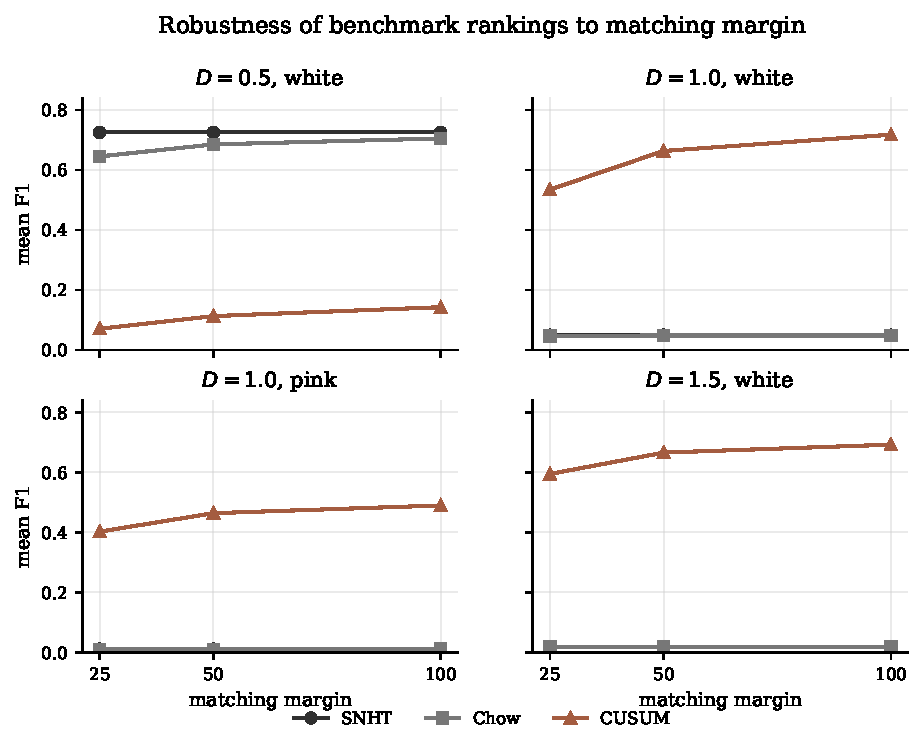
\includegraphics[width=\linewidth]{../assets/figures/fig03_matching_margin_robustness.pdf}
  \caption{Sensitivity of selected benchmark rankings to the matching margin.
  Detector outputs and post-processing are fixed; only the evaluation tolerance
  changes. The low-\(D\) and \(D=1.0\) conclusions are stable, while the
  \(D=1.5\) white-noise scenario shows the CUSUM--Transformer crossover under
  wider matching tolerances.}
  \label{fig:matching-margin-robustness}
\end{figure}


